% !TeX program = xelatex
\documentclass[aspectratio=169,10pt]{beamer}
\usepackage[UTF8,fontset=fandol]{ctex}
\usepackage{amsmath,amssymb,booktabs,tabularx,array,tikz,pgfplots,pgfpages}
\usetikzlibrary{arrows.meta,positioning}
\pgfplotsset{compat=1.18}
\linespread{1.12}
\renewcommand{\arraystretch}{1.15}

\definecolor{accent}{HTML}{28649A}
\definecolor{ink}{HTML}{17334F}
\definecolor{muted}{HTML}{596B7B}
\setbeamercolor{normal text}{fg=ink,bg=white}
\setbeamercolor{structure}{fg=accent}
\setbeamercolor{frametitle}{fg=ink}
\setbeamercolor{item}{fg=accent}
\setbeamerfont{frametitle}{size=\fontsize{13.5}{17}\selectfont,series=\bfseries}
\setbeamerfont{title}{size=\Huge,series=\bfseries}
\setbeamersize{text margin left=9mm,text margin right=9mm}
\setbeamertemplate{navigation symbols}{}
\setbeamertemplate{itemize items}[circle]
\setbeamertemplate{frametitle}{\vspace{3mm}\insertframetitle\par\vspace{1mm}\textcolor{accent}{\rule{\textwidth}{0.5pt}}}

\newcommand{\framesource}{}
\newcommand{\currentpresenter}{第 8 队}
\newcommand{\pageindicator}{\insertframenumber\,/\,\inserttotalframenumber}
\newcommand{\source}[1]{\renewcommand{\framesource}{#1}}
\newcommand{\presenter}[1]{\renewcommand{\currentpresenter}{#1}}
\setbeamertemplate{footline}{%
    \vskip2mm
    \hspace{9mm}\begin{minipage}{\dimexpr\paperwidth-18mm\relax}
        \color{muted}\fontsize{6.2}{7.5}\selectfont\framesource\par\vspace{1mm}
        \fontsize{7}{8}\selectfont\insertsectionhead\quad\currentpresenter
        \hfill\pageindicator
    \end{minipage}\vspace{2mm}}
\setbeamertemplate{note page}{\vspace{4mm}{\Large\bfseries\insertframetitle}\par\vspace{3mm}{\footnotesize\insertnote}}
\setbeameroption{hide notes}
% For presenter view, replace hide notes with show notes on second screen=right.

\newcolumntype{Y}{>{\raggedright\arraybackslash}X}
\newcommand{\key}[1]{\textcolor{accent}{\bfseries #1}}
\newcommand{\aside}[1]{\par\vspace{3mm}{\small\color{muted}#1}}
\newcommand{\takeaway}[1]{\par\vspace{4mm}{\large\bfseries #1}}
\newcommand{\papersection}[3]{%
    \section{#1}\presenter{#3}
    \begin{frame}[plain]
        \vspace{7mm}{\small\color{accent}专题论文阅读}\par
        \vspace{7mm}{\fontsize{28}{34}\selectfont\bfseries #1}\par
        \vspace{4mm}{\Large #2}\par
        \vspace{7mm}\textcolor{accent}{\rule{\textwidth}{0.8pt}}\par
        \vspace{3mm}#3\hfill 7--9 分钟
        \note{建议用约 15 秒介绍论文和讲解人。正文围绕问题、方法、证据和局限展开。}
    \end{frame}}

\hypersetup{pdftitle={长上下文场景结构化记忆建模：小组学术汇报},pdfauthor={第8队}}

% 十二页共用讲稿，供 Beamer notes 与独立讲稿引用。
\newcommand{\speechOne}{老师好，我们是第八队。课设题目是长对话结构化记忆复现与优化。今天主要介绍六篇论文怎样支撑同一研究问题，以及小组协作完成的实验和后续计划。}

\newcommand{\speechTwo}{我们研究长对话问答：根据一个人长期积累的历史，回答经历、关系和时间问题。历史很长，相关信息往往分散。同一个人多次谈旅行，检索可能找到主题相关、却属于另一次旅行的内容。“去年”又必须结合记录年份才能解释。因此，我们关注如何保留事件联系，让模型正确使用证据，同时检查结构化带来的额外成本。}

\newcommand{\speechSynthesis}{六篇论文被放进同一个分析框架：信息怎样组织、证据怎样找到、取回后怎样使用，以及更新后怎样验证。StructMem 用事件绑定和跨事件综合保留关系，是我们的实现主线。Hindsight 强调时间信息和多路检索，Semantic XPath 强调结构范围，帮助我们检查是否找对事件。MetaMem 进一步提醒，证据取到了也可能用错。HyMEM 关注经验更新，Text2Mem 关注操作及执行状态，两者帮助讨论怎样安全地维护记忆，但动态更新暂不纳入本轮实现。由此，其他论文参与定义检查维度和研究边界，而不是只在背景里列名字。它们任务和指标不同，我们也不直接拿论文分数排名。}

\newcommand{\speechThree}{具体实现分三步。先抽取事实和关系，保留说话人、来源消息和时间绑定。然后做跨事件综合：汇集一个时间窗口的新事件，检索历史种子并补齐上下文，把联系写成独立综合记忆。最后根据问题检索事件和综合条目，再交给回答模型。本轮使用一小时窗口、十五个历史种子，每题六十条事件和五条综合。事件绑定和综合来自原论文，我们完成的是适配、运行和分析。}

\newcommand{\speechFour}{实验使用 LoCoMo，固定三个开发会话、三十道题，覆盖表中的四类问题；另外七个会话留待后续评价。参考答案只在生成回答后用于评分。S 零检索六十条原始对话块；S 一只保留事件记忆；S 二再加入跨事件综合。当前阶段比较 S 零和 S 二，S 一用于后续的综合模块消融。两组公共生成参数一致，但记忆表示、输入长度和方法指令不同，因此分差描述系统对照，不能全部归因于某一个模块。}

\newcommand{\speechFive}{当前链路已经从数据贯通到评分：近两千条消息生成三千七百一十二条事件记忆，再形成九十一条综合记忆。S 零和 S 二各完成三十条真实回答，六十条裁判记录的输入指纹与分数已经离线核对。模型替换、关闭压缩等复现差异也保留记录。}

\newcommand{\speechSix}{应用既有证据裁决后，S 零答对十五题，正确率百分之五十；S 二答对十九题，正确率百分之六十三点三。多出的四题中，时间题占两题，开放域和单跳各一题，多跳相同。同时，回答输入从十三万两千多 tokens 增加到五十八万六千多，约四点四二倍，尚未计入记忆构建。原始自动裁判给 S 零十六题正确，其中一条日期回答存在矛盾，经证据复核改为错误，所以正文显示十五题。原始判定和后续裁决分别保留。这些结果只描述固定三十道开发题，还不能证明稳定提升。}

\newcommand{\speechSeven}{用同一个旅行案例，可以把几篇论文的视角连起来。消息记录于二零二三年四月十日，内容说的是“我们去年进行的公路旅行”，相关对话确认了地点。S 零把记录日期当成旅行日期；S 二回答去年，也就是二零二二年。StructMem 关注人物、地点和事件的联系；Hindsight 提醒区分记录时间与发生时间；MetaMem 提醒检查取回的证据是否用对。这里是在用多篇论文共同分析一个真实结果，并不意味着已经实现它们的全部机制，也不能仅凭这一个案例断定改进原因。}

\newcommand{\speechEight}{文献比较与现有结果共同指向下一步：先弄清收益来自哪里，再控制输入成本。首先开展 S 一消融，在事件库、模型和方法指令一致的条件下，只关闭跨事件综合。其次把事件检索数从六十减到三十，综合记忆仍取五条，观察质量和输入量如何变化。如果下降也如实保留。开发集确定配置以后，再从七个留出会话分层抽取约一百题评价。动态更新和基于反馈的规则学习暂不扩展，先把当前问题做扎实。以上都是待运行方案。}

\newcommand{\speechNine}{六人分工围绕同一条链路衔接。A 冻结数据、划分和题单；B 提供普通检索；C 交付事件记忆；D 接着生成综合记忆并完成 S 二；E 评分和分析；F 提供统一回答接口，完成 S 零、联调与复算。连接这些工作的是同一题单、统一输入输出和逐题来源记录。这里不仅有任务划分，也有下游接收与交叉核查。表中列出的是目前大致贡献。}

\newcommand{\speechCollaboration}{我们主要通过 GitHub、微信群和线下讨论协作。GitHub 用来管理任务、代码和文档，通过 Issue 和 PR 记录进展、交接和修改；微信群用于日常沟通、同步进度，及时协调接口、数据和材料问题；线下则集中讨论论文之间的联系、实验方案、结果分析和汇报内容。六位同学虽然负责不同模块，但始终围绕同一个研究问题、同一批题目和同一条实验链路推进，并在交接时相互核对。这样，个人阅读和实现能够汇入共同的分析与实验。}

\newcommand{\speechTen}{最后，我们用共同问题组织六篇论文，再围绕同一实验链路分工、交接和核查。现有结果是 S 二多答对四题，回答输入约四点四二倍。下一步开展综合模块消融和预算对照，并通过留出评价，形成可复跑、有证据的结论。}

\linespread{1.08}
\setbeamerfont{frametitle}{size=\fontsize{15}{19}\selectfont,series=\bfseries}
\setbeamerfont{normal text}{size=\fontsize{10}{14}\selectfont}
\renewcommand{\pageindicator}{\insertframenumber\,/\,12}
\setbeamertemplate{footline}{%
  \hfill{\color{ink}\fontsize{8}{10}\selectfont\pageindicator}\hspace{9mm}\vspace{2mm}}
\hypersetup{pdftitle={长对话结构化记忆复现与优化：8分钟研讨汇报},pdfauthor={NLP 第8队}}
\begin{document}

\source{依据：项目方案（2026-10-21）；本组固定开发集实验与评分复算记录。}
\begin{frame}[plain]
  \vspace{5mm}
  {\color{accent}\large 天津大学自然语言处理课程设计\par}
  \vspace{6mm}
  {\fontsize{24}{31}\selectfont\bfseries 长对话结构化记忆\par 复现与优化\par}
  \vspace{4mm}
  {\large StructMem 方法复现与固定开发集初步分析\par}
  \vspace{6mm}
  \textcolor{accent}{\rule{\linewidth}{0.7pt}}\par\vspace{3mm}
  第 8 队\hfill 第一次课设研讨 · 2026 年 10 月 22 日\par
  \note{\speechOne\par\medskip 来源：\framesource}
\end{frame}

\source{依据：StructMem 原文第 2--3 页、图 2；本组项目方案第 1、3 节。}
\begin{frame}[t]{研究问题：长对话中的事件证据如何被正确使用}
  \vspace{1mm}
  \textbf{任务：}给定一个人的长期对话历史，回答与其经历、关系和时间有关的问题。\par
  \vspace{3mm}
  \begin{itemize}\setlength{\itemsep}{2.5mm}
    \item \key{历史很长，相关信息分散。}同一人物会多次谈到相似活动，仅按关键词或语义相似度检索，可能找到另一件事。
    \item \key{事实有关联，时间有参照。}“谁、何时、做了什么”需要一起保留；“去年”的含义还依赖消息的记录日期。
    \item \key{结构更丰富，也可能更昂贵。}额外抽取和综合需要模型调用，回答时输入的记忆也可能明显增多。
  \end{itemize}
  \vspace{3mm}
  \textbf{本组研究问题：}结构化记忆能带来怎样的回答变化？这些变化需要付出多少输入与构建成本？
  \note{\speechTwo\par\medskip 来源：\framesource}
\end{frame}

\source{依据：notes/six-paper-comparison.md；reports/homework/sections/07-synthesis.tex。StructMem pp.2--3 Fig.2；Hindsight pp.2--5 Fig.1；Semantic XPath pp.2--5 Fig.2；MetaMem pp.3--5 Fig.2；HyMEM pp.3--5 Fig.1；Text2Mem pp.3--5 Fig.2/Table 1。}
\begin{frame}[t]{六篇论文的共同主线：记忆怎样变成可靠答案}
  \vspace{1mm}
  \textbf{统一分析链条：}\key{组织信息 $\rightarrow$ 找对证据 $\rightarrow$ 正确使用 $\rightarrow$ 更新与验证}\par
  \vspace{4mm}
  \begingroup
  \fontsize{9.1}{12.2}\selectfont
  \renewcommand{\arraystretch}{1.04}
  \begin{tabularx}{\linewidth}{@{}p{20mm}>{\raggedright\arraybackslash}p{44mm}Y@{}}
    \toprule 共同问题 & 相互补充的论文视角 & 对本组方案的具体作用\\\midrule
    关系如何保留 & StructMem：事件绑定与综合 & 选作实现主线，保存人物、时间和来源关系。\\[1.2mm]
    范围是否正确 & Hindsight：时间与多路检索\newline Semantic XPath：层级范围 & 检查记忆是否来自正确会话，区分记录时间与事件时间。\\[1.2mm]
    证据是否用对 & MetaMem：知识利用经验 & 将“没取到证据”与“取到但用错”分开分析。\\[1.2mm]
    更新能否验证 & HyMEM：经验更新\newline Text2Mem：操作验证 & 比较更新策略与验证要求；动态更新留作后续研究。\\
    \bottomrule
  \end{tabularx}\par
  \endgroup
  \vspace{4mm}
  \textbf{本组取舍：}StructMem 为实验主线，其他论文提供诊断与验证视角。
  \note{\speechSynthesis\par\medskip 来源：\framesource}
\end{frame}

\source{方法来源：StructMem 第 2--3 页、图 2；第 8 页附录参数。实现依据：C 事件记忆、D 综合与检索交接。}
\begin{frame}[t]{StructMem：把事件关系与跨事件联系保留下来}
  \vspace{3mm}
  \begin{tabularx}{\linewidth}{@{}p{25mm}Y@{}}
    \toprule
    步骤 & 本组采用的处理方式\\\midrule
    \key{1. 抽取与绑定} & 分别抽取事实和关系，保留说话人、来源消息与时间绑定。相关条目可以追溯到原始事件。\\[2mm]
    \key{2. 跨事件综合} & 汇集一个时间窗口内的新事件，检索历史种子并补齐事件上下文，再生成单独保存的综合记忆。\\[2mm]
    \key{3. 检索与回答} & 问题到来时，检索事件条目和综合记忆，再交给回答模型；最终保留预测、来源与 token 用量。\\
    \bottomrule
  \end{tabularx}\par
  \vspace{4mm}
  \textbf{本次参数：}1 小时综合窗口，15 个历史种子；每题取 60 条事件记忆和 5 条综合记忆。\par
  \note{\speechThree\par\medskip 来源：\framesource}
\end{frame}

\source{依据：项目方案第 3 节；A 固定题单；S0/S2 回答配置；统一回答与联调说明。}
\begin{frame}[t]{实验设计：固定题集，比较两套已完成的系统}
  \vspace{1mm}
  \textbf{数据：}LoCoMo 固定 3 个开发会话、30 道题；四类题数量为 8/8/7/7。\par
  \vspace{1mm}
  另留 7 个会话供后续评价；标准答案单独保存，只在生成回答后用于评分。\par
  \vspace{4mm}
  \begin{tabularx}{\linewidth}{@{}p{14mm}Yp{24mm}@{}}
    \toprule 方法 & 每道题的回答输入 & 进展\\\midrule
    S0 & 原始对话块的向量检索，取前 60 条 & 已完成 30 题\\[2mm]
    S1 & 事件记忆，关闭跨事件综合 & 后续消融\\[2mm]
    S2 & 60 条事件记忆 + 5 条综合记忆 & 已完成 30 题\\
    \bottomrule
  \end{tabularx}\par
  \vspace{4mm}
  \textbf{公共条件：}DeepSeek-Flash、非思考模式、temperature=0；本地 MiniLM 嵌入。\par
  \note{\speechFour\par\medskip 来源：\framesource}
\end{frame}

\source{依据：C development-complete、D real-run；S0/S2 回答交接；2026-10-21 评分复算与 C 对 D 的核查记录。}
\begin{frame}[t]{实际进展：数据、记忆、回答与评分已经贯通}
  \vspace{3mm}
  \begin{tabularx}{\linewidth}{@{}p{24mm}Y@{}}
    \toprule 阶段 & 已完成的真实产物\\\midrule
    数据与基线 & 3 个开发会话，91 个 session 时段，1,973 条原始消息；S0 完成固定 30 题检索。\\[0.5mm]
    事件记忆 & 3,712 条事件记忆，其中 2,309 条事实、1,403 条关系；保留来源绑定。\\[0.5mm]
    综合与回答 & 91 条综合记忆；S0 与 S2 各完成 30 条真实回答，生成记录均已核验。\\[0.5mm]
    评分与复核 & 60 条自动裁判记录；已核对 60 个输入指纹并离线复算，分类分数与汇总一致。\\
    \bottomrule
  \end{tabularx}\par
  \note{\speechFive\par\medskip 来源：\framesource}
\end{frame}

\source{数据：e-score-verification-20261021.json；e-score-20261020.md。分母固定为 30；用量仅指回答阶段。}
\begin{frame}[t]{开发集结果：S2 多答对 4 题，输入约为 4.42 倍}
  \vspace{1mm}
  \begin{columns}[T,onlytextwidth]
    \begin{column}{0.60\textwidth}
      \textbf{应用既有证据裁决后的正确数}\par\vspace{3mm}
      \renewcommand{\arraystretch}{1.02}
      \begin{tabularx}{\linewidth}{@{}Yrr@{}}
        \toprule 题型 & S0 & S2\\\midrule
        多跳（8 题） & 4/8 & 4/8\\
        时间（8 题） & 5/8 & 7/8\\
        开放域（7 题） & 2/7 & 3/7\\
        单跳（7 题） & 4/7 & 5/7\\\midrule
        \textbf{总体（30 题）} & \textbf{15/30} & \textbf{19/30}\\
        \textbf{正确率} & \textbf{50.0\%} & \textbf{63.3\%}\\
        \bottomrule
      \end{tabularx}\par
    \end{column}
    \begin{column}{0.36\textwidth}
      \textbf{回答输入（千 tokens）}\par\vspace{3mm}
      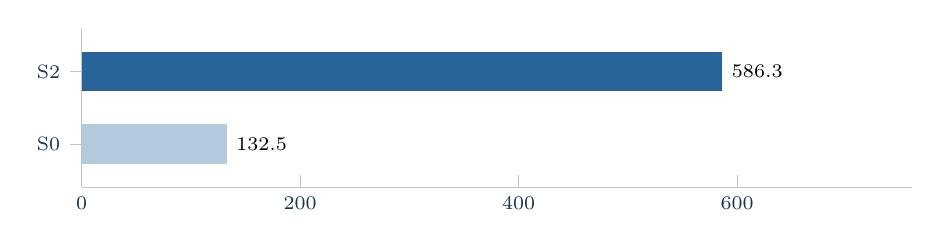
\begin{tikzpicture}
        \begin{axis}[width=\linewidth,height=36mm,xbar,bar width=5mm,
          xmin=0,xmax=760,xtick={0,200,400,600},ytick={0,1},yticklabels={S0,S2},
          ymin=-0.6,ymax=1.6,axis x line*=bottom,axis y line*=left,
          tick label style={font=\scriptsize,color=ink},
          axis line style={muted!40},tick style={muted!40},
          nodes near coords,point meta=x,
          nodes near coords style={font=\scriptsize,/pgf/number format/fixed,/pgf/number format/precision=1},
          clip=false]
          \addplot[fill=accent!35,draw=none,bar shift=0pt] coordinates {(132.531,0)};
          \addplot[fill=accent,draw=none,bar shift=0pt] coordinates {(586.282,1)};
        \end{axis}
      \end{tikzpicture}\par
      {\small S0：132,531 tokens\par S2：586,282 tokens}
    \end{column}
  \end{columns}
  \vspace{4mm}
  原始自动裁判为 S0 16/30、S2 19/30；一条日期回答经证据复核后改判。\par
  \vspace{2mm}
  \textbf{结论范围：}30 道开发题的系统对照，尚不能证明稳定提升。\par
  \note{\speechSix\par\medskip 来源：\framesource}
\end{frame}

\source{案例：conv-41/20，原始消息 D11:3 与 D11:5；conv-42/28，D16:8。见六例复核与来源索引。}
\begin{frame}[t]{案例：记录日期与事件发生时间需要区分}
  \vspace{1mm}
  \textbf{问题：}John 什么时候去太平洋西北地区进行公路旅行？\par
  \vspace{1.5mm}
  \textbf{原始证据：}消息记录于 \key{2023 年 4 月 10 日}，其中说：\par
  \vspace{1mm}
  \hspace{4mm}“\textit{a road trip we took last year}”\quad（节选）\par
  {\small\hspace{4mm}相关对话同时确认了旅行地点。}\par
  \vspace{4mm}
  \begin{tabularx}{\linewidth}{@{}p{14mm}p{43mm}Y@{}}
    \toprule 系统 & 实际回答 & 证据解释\\\midrule
    S0 & 10 April, 2023 & 把消息记录日期作为旅行日期。\\[1.5mm]
    S2 & Last year (2022) & 将“去年”与记录年份对应，得到 2022 年。\\
    \bottomrule
  \end{tabularx}\par
  \vspace{4mm}
  \textbf{同一案例，贯通三种视角：}StructMem 保留事件联系；Hindsight 提醒区分两种时间；MetaMem 提醒检查证据是否被正确使用。\par
  \note{\speechSeven\par\medskip 来源：\framesource}
\end{frame}

\source{依据：项目方案第 6--7 节。以下为待验证的研究方案，未计入当前实验结果。}
\begin{frame}[t]{创新性论证与后续方案}
  \vspace{1mm}
  \textbf{已完成的工作：}适配并运行 StructMem，建立统一题集的系统对照，记录来源、用量与错误案例。\par
  \vspace{3mm}
  \begin{itemize}\setlength{\itemsep}{2.3mm}
    \item \key{先检验综合模块的作用。}开展 S1 消融，与 S2 共享事件库、回答模型和方法指令，只关闭跨事件综合，观察分类正确率和输入变化。
    \item \key{再检验检索预算。}将事件条目数从 60 调为 30，综合记忆仍为 5 条，检查能否在质量接近时减少回答输入。
    \item \key{最后评价泛化。}开发集上确定配置后，再从留出会话分层抽取约 100 题；保留失败和负结果，不看成绩临时换题。
  \end{itemize}
  \note{\speechEight\par\medskip 来源：\framesource}
\end{frame}

\source{分工依据：项目方案第 8 节与各成员交接。目前大致贡献按每人 1/6 展示。}
\begin{frame}[t]{六人分工：围绕同一条实验链路交接}
  \vspace{3mm}
  \begingroup
  \fontsize{8.6}{11.5}\selectfont
  \setlength{\tabcolsep}{3pt}
  \renewcommand{\arraystretch}{1.12}
  \begin{tabularx}{\linewidth}{@{}p{35mm}Yp{22mm}@{}}
    \toprule 任务 / 成员账号 & 已完成的工作 & 目前大致贡献\\\midrule
    A\quad ngocnamd93-spec & 冻结数据、开发/留出划分与题单；隔离答案，准备嵌入环境。 & $1/6$\\[0.6mm]
    B\quad YaoYang-123456 & 实现原始对话块的 top-60 检索；完成固定题集检索与 MetaMem 阅读。 & $1/6$\\[0.6mm]
    C\quad oioioi-521 & 完成事实/关系抽取、事件绑定与持久化，交付 3,712 条事件记忆。 & $1/6$\\[0.6mm]
    D\quad lanshuheng9-oss & 生成 91 条综合记忆；完成 S2 检索与 30 题回答。 & $1/6$\\[0.6mm]
    E\quad onlysonder & 完成 60 条自动评分、分类汇总与案例复核材料，交接逐题记录。 & $1/6$\\[0.6mm]
    F\quad hycx233 & 提供统一回答入口，完成 S0 回答、接口联调、评分复算与材料整合。 & $1/6$\\
    \bottomrule
  \end{tabularx}\par
  \endgroup
  \note{\speechNine\par\medskip 来源：\framesource}
\end{frame}

\source{依据：docs/collaboration.md；本轮用户确认主要通过 GitHub 协作、微信群和线下讨论推进。}
\begin{frame}[t]{协作方式：GitHub、微信群与线下讨论}
  \vspace{2mm}
  \begin{itemize}\setlength{\itemsep}{5mm}
    \item \key{GitHub：管理任务与共同产物。}\par
      通过 Issue 和 PR 组织分工、代码与文档，记录进展、交接、审核和修改。
    \item \key{微信群：日常沟通与进度同步。}\par
      及时沟通接口、数据和材料问题，协调成员之间的交接与安排。
    \item \key{线下讨论：集中梳理与交流。}\par
      围绕论文之间的联系、实验方案、结果分析和汇报内容进行讨论。
  \end{itemize}
  \vspace{4mm}
  \textbf{协作重点：}围绕同一研究问题，对齐论文理解、实验方案与汇报内容。
  \note{\speechCollaboration\par\medskip 来源：\framesource}
\end{frame}

\source{依据：截至 2026-10-21 的项目方案、评分复算记录与真实交接材料。}
\begin{frame}[t]{阶段结论与下一步}
  \vspace{2mm}
  \begin{enumerate}\setlength{\itemsep}{4mm}
    \item \key{用共同问题组织论文，用共同产物串联分工。}\par
      六篇论文提炼为统一分析框架；成员围绕同一题集、记忆库、回答与评分交接，并交叉核查。
    \item \key{观察到质量变化，也看到了输入代价。}\par
      应用既有证据裁决后，S0 为 15/30，S2 为 19/30；S2 的回答输入约为 S0 的 4.42 倍。
    \item \key{下一步明确收益来自哪里、能否降低成本。}\par
      开展 S1 消融与检索预算对照，并在留出题集上检验泛化表现。
  \end{enumerate}
  \vspace{4mm}
  \textbf{预期交付：}可复跑的配置与代码、结果表、成本记录，以及有原文依据的案例分析。
  \note{\speechTen\par\medskip 来源：\framesource}
\end{frame}
\end{document}
